\documentclass[10pt]{article}
\usepackage[ngerman]{babel}
\usepackage[utf8]{inputenc}
\usepackage[T1]{fontenc}
\usepackage{amsmath}
\usepackage{amsfonts}
\usepackage{amssymb}
\usepackage[version=4]{mhchem}
\usepackage{stmaryrd}
\usepackage{graphicx}
\usepackage[export]{adjustbox}
\graphicspath{ {./images/} }
\usepackage{fvextra, csquotes}

\begin{document}
\section*{CT1 Übungsaufgaben}
\section*{Exceptional Control Flow}
\section*{Aufgabe 1}
Um eine Interrupt Quelle nutzen zu können muss der entsprechende Interrupt enabled werden (neben anderen Konfigurationsaktionen).

Annahme: Sie müssen für den Timer 2 einen Handler installieren und den Interrupt enablen.

\begin{enumerate}
  \item Wie heisst der Interrupt Handler für Timer 2?
\end{enumerate}

Öffnen Sie dazu in irgendeinem der Praktika Projekte das File startup\_ctboard.s und suchen sie nach dem passenden Handler Namen in der $\qquad$ Vectors Tabelle.\\
Tipp: Suchen Sie nach TIM2...\\
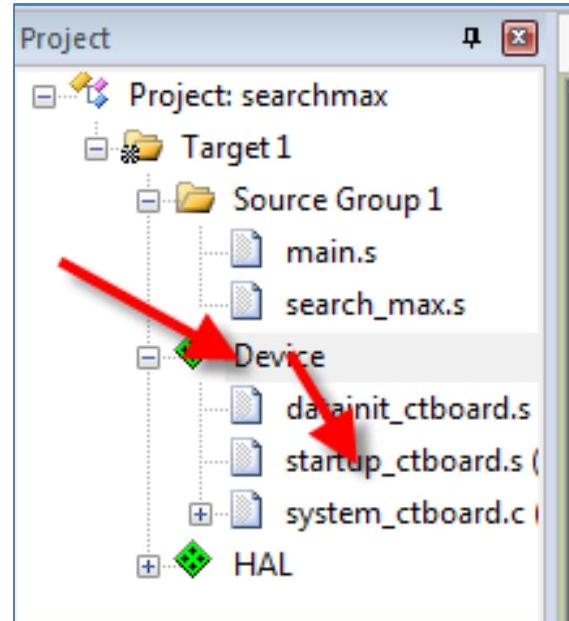
\includegraphics[width=\linewidth]{images/2025_01_02_1e89fec346403e1ae751g-1}

\section*{TIM2\_IRQHandler}
\begin{enumerate}
  \setcounter{enumi}{1}
  \item Welche Interrupt Nummer hat dieser externe Interrupt? Zählen Sie vom ersten externen Interrupt, beginnend mit 0, bis zum entsprechenden Interrupt Handler.
\end{enumerate}

28\\
3) Geben Sie die Assembler Instruktionen an um diesen Interrupt mit der gegebenen Interrupt Nummer zu enablen - siehe Vorlesung Seite 27: „Interrupt Enable Registers".

\begin{verbatim}
SETENAO EQU OxEOOOE100
    LDR R7,=SETENAO
    MOVS R6,#1
    LSLS R6,#28
    STR R6,[R7]
\end{verbatim}

\section*{Aufgabe 2}
Enabling von Interrupt Quellen, wie in Aufgabe 1 behandelt, dient zur initialen Konfiguration von Interrupts. Im Betrieb ist es aber unter Umständen nötig alle Interrupts kurzfristig auszuschalten und danach wieder einzuschalten.

\begin{enumerate}
  \item Was kann ein Grund sein für ein solches kurzfristiges Aus- und wieder Einschalten?
\end{enumerate}

Data Konsistenz: z.B. eine Interrupt Service Routine eines Timers unterhält zwei Zähler,\\
einen für Minuten und einen für Stunden. Beim Übergang von Minute 59 zu 0 wird der

Stundenzähler um eins erhöht. Eine andere Routine welche diese beiden Zähler ausliest\\
muss dafür sorgen dass kein Interrupt passiert zwischen dem Zugriff auf diese beiden Zähler.\\
2) Wie schalten Sie alle Interrupts in Assembler aus? Wie ein?

Ausschalten:

\begin{displayquote}
CPSID i
\end{displayquote}

Einschalten:\\
CPSIE i\\
3) Wie schalten Sie alle Interrupts in C aus? Wie ein?

Ausschalten:

\begin{verbatim}
_disable_irq();
\end{verbatim}

Einschalten:

\begin{verbatim}
    __enable_irq();
\end{verbatim}

\section*{Aufgabe 3}
Der ARM Prozessor rettet beim Abarbeiten eines Interrupts gewisse Register auf den Stack bevor die ISR (Interrupt Service Routine) ausgeführt wird - und restauriert diese nach Beendigung der ISR automatisch.

\begin{enumerate}
  \item Wenn Sie in Ihrer ISR die Register R0-R6 verwenden, welche dieser Register müssen Sie auf den Stack pushen weil sie nicht schon automatisch vorher gerettet wurden?
\end{enumerate}

\begin{verbatim}
PUSH {R4-R6} ; R0-R3 wurden schon automatisch gerettet
\end{verbatim}

\begin{enumerate}
  \setcounter{enumi}{1}
  \item Wie Unterscheidet sich in der Programmierung eine ISR von einer „normalen" Funktion?
\end{enumerate}

Jede ISR hat einen vordefinierten Namen (von der $\qquad$ Vectors Tabelle vorgegeben).

Eine ISR kann keine Werte zurückgeben (ist in C eine void iss\_name (void) Funktion).

Eine ISR muss gegebenenfalls den Interrupt zurücksetzen so dass er nicht permanent feuert.


\end{document}